
\chapter{Introduction}
 
 {\slshape \scshape ``You have to be in a state of play to design. If you're not in a state of play, you can't build anything." - Paula Scher}

Mechatronics is an amalgam of "mechanisms" and "electronics": systems that contain both mechanical and electrical components. It's a field that spans nearly every industry, so any one source (even this one) will not be complete with all the information you need. But this may be a good jumping off point. I'm writing this generally towards those in a competitive robotics environment, so will use many examples from there, but you soon find that those same technologies that shoot foam balls into goals can be used anywhere from assembly lines to emergency medical equipment or racecars.

This document is not intended to be all-encompassing. In reality, it's just an outline; a map. We live in an era where information is readily available on demand. This document really doesn't contain anything new. Its goal is to show you a plethora of things that exist in a breadth-first fashion before you dive down a particular rabbit hole. There are a few places where I'll dive deeper because I feel it's relevant to show you some of the nuances you should be aware of. By and large, my goal isn't to drill home every single thing because I'll fail at that and fail you in the process. Someone will come up with something new, or improve something discussed here, and this information will become outdated. I'll try to keep it up to date... but I will definitely fail!

Some sections of this will be dry... The human mind is a weird thing. It's better at prompted recall than unprompted recall. You may not always be thinking about the many different types of bolts, but if you've seen one before, and you come across a problem that needs it, you might be able to figure it out - or at least know where to start looking.

I hope to keep this terse. We're going to go fast and I'm going to leave some things to your imagination or research to figure out exactly how they work. I love mechatronics and hope you do too, so I don't want to spoil it by chewing your steak for you.

\begin{mdframed}[style=QuestionBox]
	I'll ask some questions in boxes like these. The answers won't be in this text! It shouldn't be critical for you to know,either, but if you are so inclined, do some additional research and you'll learn more.
\end{mdframed}

With that... let's begin.

\chapter{Terminology}

Engineers use a lot of nomenclature. While some nomenclature is windowdressing, most of it in engineering is useful in saying exactly what you mean. If you've been through physics, or hung around engineers enough, most of these terms should be self-explanatory. Skim through this section- and use it like a glossary if you come across a word you don't know.

\section{Stresses and Deformations}
We use these terms to denote the shape of material deformation (indicated by the dashed lines and solid shapes), or the direction which a load is applied (indicated by the arrows). Buckling is a special phenomenon in which a compressive force causes a bending-like deformation.
\begin{figure}[H]
\begin{subfigure}[b]{.32\linewidth}
	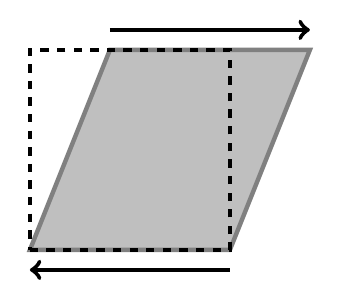
\begin{tikzpicture}[x=1.0in, y=1.0in]
	  %\fill[lightgray] (1.0,0)--(0,1.0)--(0,0)--cycle;
	  \filldraw[color=gray, fill=lightgray, ultra thick] (0,0) -- (1,0) -- (1.4,1) -- (0.4,1) -- cycle;
	  \draw[black, ultra thick, dashed] (0,0) -- (1,0) -- (1.0,1) -- (0.0,1) -- cycle;
	  \draw[black, ->, ultra thick] (1,-0.1) -- (0,-0.1);
	  \draw[black, ->, ultra thick] (0.4,1.1) -- (1.4,1.1);
	\end{tikzpicture}
	\caption{Shear}
\end{subfigure}\begin{subfigure}[b]{.32\linewidth}
	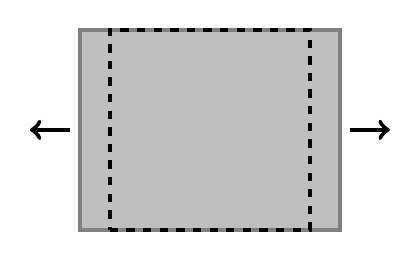
\begin{tikzpicture}[x=1.0in, y=1.0in]
	  %\fill[lightgray] (1.0,0)--(0,1.0)--(0,0)--cycle;
	  \filldraw[color=gray, fill=lightgray, ultra thick] (-0.15,0) -- (1.15,0) -- (1.15,1) -- (-0.15,1) -- cycle;
	  \draw[black, ultra thick, dashed] (0,0) -- (1,0) -- (1.0,1) -- (0.0,1) -- cycle;
	  \draw[black, ->, ultra thick] (-0.2,0.5) -- (-0.4,0.5);
	  \draw[black, ->, ultra thick] (1.2,0.5) -- (1.4,0.5);
	  \draw[black, ->, ultra thick, opacity=0] (1,-0.1) -- (0,-0.1);
	\end{tikzpicture}
	\caption{Axial / Tension}
\end{subfigure}\begin{subfigure}[b]{.32\linewidth}
	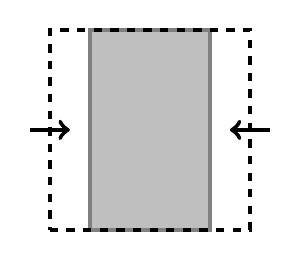
\begin{tikzpicture}[x=1.0in, y=1.0in]
	  %\fill[lightgray] (1.0,0)--(0,1.0)--(0,0)--cycle;
	  \filldraw[color=gray, fill=lightgray, ultra thick] (0.2,0) -- (0.8,0) -- (0.8,1) -- (0.2,1) -- cycle;
	  \draw[black, ultra thick, dashed] (0,0) -- (1,0) -- (1.0,1) -- (0.0,1) -- cycle;
	  \draw[black, <-, ultra thick] (0.1,0.5) -- (-0.1,0.5);
	  \draw[black, <-, ultra thick] (0.9,0.5) -- (1.1,0.5);
	  \draw[black, ->, ultra thick, opacity=0] (1,-0.1) -- (0,-0.1);
	\end{tikzpicture}
	\caption{Axial / Compression}
\end{subfigure}

\begin{subfigure}[b]{.47\linewidth}
	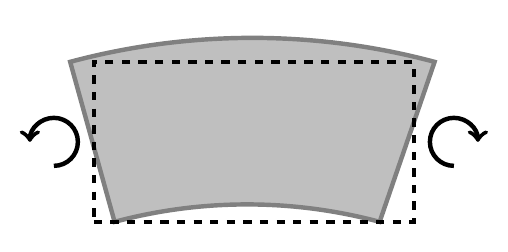
\begin{tikzpicture}[x=0.8in, y=0.8in]
	  %\fill[lightgray] (1.0,0)--(0,1.0)--(0,0)--cycle;
	  \filldraw[color=gray, fill=lightgray, ultra thick] ({0.5*sin(15)},-0.5) arc(105:75:3.2) -- ({2+0.5*sin(15)},0.5) arc(75:105:4.4) -- cycle;
	  \draw[black, ultra thick, dashed] (0,-0.5) -- (2,-0.5) -- (2,0.5) -- (0,0.5) -- cycle;
	  \draw[black, <-, ultra thick] (-0.4,0) arc(180:-90:0.15);
	  \draw[black, <-, ultra thick] (2.4,0) arc(0:270:0.15);
	\end{tikzpicture}
	\caption{Bending}
\end{subfigure}\begin{subfigure}[b]{.47\linewidth}
	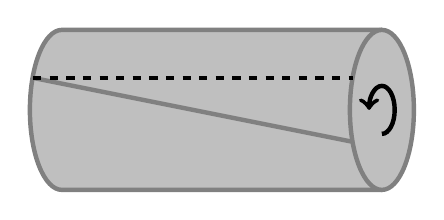
\begin{tikzpicture}[x=0.8in, y=0.8in]
	  \filldraw[color=gray, fill=lightgray, ultra thick] (2,-0.5) -- (0,-0.5) arc (270:90:0.2 and 0.5) -- (2,0.5);
	  \filldraw[color=gray, fill=lightgray, ultra thick] (2,0) circle[x radius=0.2, y radius=0.5];
	  \draw[color=gray, ultra thick] (-0.18, 0.2) -- (1.82, -0.2);
	  \draw[color=black, ultra thick, dashed] (-0.18, 0.2) -- (1.82, 0.2);
	  %\draw[black, <-, ultra thick] (-0.3,0) arc(0:270:0.08 and 0.15);
	  \draw[black, <-, ultra thick] (1.92,0) arc(180:-90:0.08 and 0.15);
	\end{tikzpicture}
	\caption{Torsion}
\end{subfigure}

\begin{subfigure}[b]{.95\linewidth}
	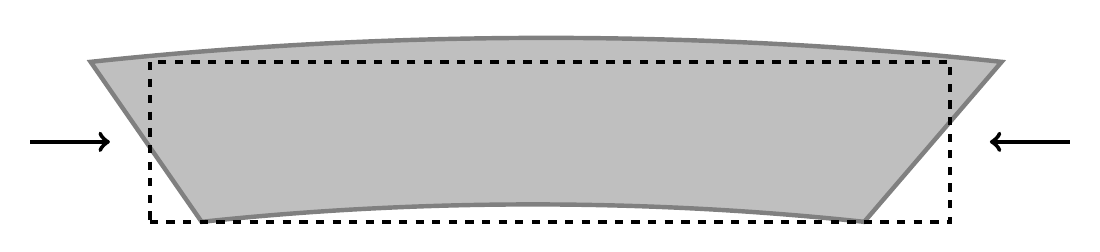
\begin{tikzpicture}[x=2.0in, y=0.8in]
	  %\fill[lightgray] (1.0,0)--(0,1.0)--(0,0)--cycle;
	  \filldraw[color=gray, fill=lightgray, ultra thick] ({0.5*sin(15)},-0.5) arc(105:75:3.2) -- ({2+0.5*sin(15)},0.5) arc(75:105:4.4) -- cycle;
	  \draw[black, ultra thick, dashed] (0,-0.5) -- (2,-0.5) -- (2,0.5) -- (0,0.5) -- cycle;
	  \draw[black, <-, ultra thick] (-0.1,0) -- (-0.3,0);
	  \draw[black, <-, ultra thick] (2.1,0) -- (2.3,0);
	\end{tikzpicture}
	\caption{Buckling}
\end{subfigure}

\end{figure}

\section{Directions and Coordinate Systems}
\begin{figure}[H]
\includegraphics[width=0.8\textwidth]{imgs/radial_axial.png}
\caption{Axial vs. radial directions.}
\end{figure}

The axial direction is along the axis of symmetry for a shaft, or along the axis of rotation for a rotating component.
The radial direction(s) are perpindicular to this axis of symmetry, and coincide at a point, emanating outwards.
The tangential direction(s) are perpindicular to both the radial and axial directions, curving around the axis of rotation.

\textit{Orthogonal} is a synonym for \textit{perpindicular}; at 90 degrees to.
An axis may be \textit{normal} to a plane if it is perpindicular in two directions.
If the plane and axis have specified positive directions, it may be \textit{antinormal} if the positive directions are opposed to each other.
Axes and planes may be \textit{parallel} to each other.
Axes and planes may be \textit{antiparallel} to each other if the positive directions are opposed to each other.
A surface (with nonzero curvature) can be \textit{tangent} to a line or another surface.

\textit{Mass} ($m$) is the amount of matter an object has.
\textit{Force} ($F$) is motive for objects to change velocity.
\textit{Acceleration} ($a$) is a change in an object's velocity over time.
\textit{Velocity} ($v$) is a change in an object's position over time.
\textit{Position} ($x$) is an object's location in space.
These three ideas are summed up in the equation of

\begin{equation}
	\vec{F_{net}} = m \times \vec{a}
\end{equation}

(for rigid objects which do not change mass). You may ask why the $\vec{F}$ and $\vec{a}$ have that little arrow over the top of them. That's to denote that they are \textit{vectors}; they have multiple components. You can break this equation down simply into

\begin{equation}
	F_x = m \times a_x \\
	F_y = m \times a_y \\
	F_z = m \times a_z
\end{equation}

which lets you see that simply exerting a force on an objet will cause it to accelerate in that given direction. If it has more mass, it will accelerate less.

These concepts exist in an analogue for rotating components as well.

\textit{Moment of inertia} or \textit{MOI} ($I$) is a measure of how spread out an object's mass is. A point mass (black hole) has a MOI of zero. A golf ball would have a small MOI, and a beach ball would have a large MOI, even if the beach ball has less mass.
\textit{Torques} or \textit{Moments} ($T$ or $M$) are twisting forces. They can be quantified by how much force is applied multiplied by the lever arm which it is applied by.
\textit{Angular acceleration, velocity, and positions} ($\alpha$, $\omega$, $\theta$) are just like their linear counterparts, except they are measured as rotation about an axis.

\begin{equation}
	\vec{M} = \frac{d}{dt} [I] \vec{\omega}
\end{equation}

(which again holds for rigid objects). You may ask why the moment of inertia $[I]$ has those brackets around it. That's to denote that it's a \textit{matrix}. This means that breaking the equation down is difficult if there are multiple rotations. The \frac{d}{dt} is a derivative, concept from calculus. Luckily, for the simple case of an object of constant moment of inertia, and spinning only about one axis $x$,

\begin{equation}
	M_x = I_x \alpha_x
\end{equation}

which isn't so scary, and is just like the linear case.

\textit{Energy} is a property that can be transformed in many ways to do useful \textit{work}. There are many forms of energy (spring, gravitational, electrical, chemical) and many different processes that can be used to transform it (combustion, releasing a spring, lifting a heavy object).